% Created 2018-09-26 Wed 21:07
% Intended LaTeX compiler: pdflatex
\documentclass[journal=ancac3,manuscript=article,email=true,hyperref=true,keywords=false]{achemso}
\usepackage[utf8]{inputenc}
\usepackage{graphicx}
\usepackage{float}
\usepackage{xcolor}
\usepackage{amsmath}
\usepackage{amssymb}
\usepackage{lineno}
\usepackage{todonotes}
\usepackage{times}

%\usepackage{xr}
\usepackage{xr-hyper} 
\externaldocument[SI-]{SI}



\author{Tian Tian}
\affiliation{Institute for Chemical and Bioengineering, ETH Z{\"{u}}rich,  Vladimir Prelog Weg 1, CH-8093 Z{\"{u}}rich, Switzerland}
\altaffiliation{T. T. and D. S. contributed equally to this work}
\author{Declan Scullion}
\affiliation{School of Mathematics and Physics, Queen's University Belfast, BT7 1NN, United Kingdom}
\altaffiliation{T. T. and D. S. contributed equally to this work}
\author{Dale Hughes}
\affiliation{School of Mathematics and Physics, Queen's University Belfast, BT7 1NN, United Kingdom}
\author{Lu Hua Li}
\affiliation{Institute for Frontier Materials, Deakin University, Waurn Ponds, Victoria, Australia}
\author{Chih-Jen Shih}
\affiliation{Institute for Chemical and Bioengineering, ETH Z{\"{u}}rich,  Vladimir Prelog Weg 1, CH-8093 Z{\"{u}}rich, Switzerland}
\author{Jonathan Coleman}
\affiliation{School of Physics, Centre for Research on Adaptive Nanostructures and Nanodevices (CRANN) and Advanced Materials and BioEngineering Research (AMBER), Trinity College Dublin, Dublin 2, Ireland.}
\author{Manish Chhowalla}
%% \affiliation{Materials Science and Engineering, Rutgers University, 607 Taylor Road, Piscataway, New Jersey 08854, USA.}
\affiliation{Department of Materials Science \& Metallurgy, University of Cambridge, CB3 0FS, United Kingdom}
\author{Elton J. G. Santos}
\email{e.santos@qub.ac.uk}
\affiliation{School of Mathematics and Physics, Queen's University Belfast, BT7 1NN, United Kingdom}
\date{}
\title{Electronic polarizability as the fundamental variable in the dielectric properties of two-dimensional materials}
%\title{The Unified Nature of the Dielectric Properties of Two-Dimensional Materials}
% \title{Unified Understanding of the Dielectric Nature of Two-Dimensional Materials}

\keywords{Dielectric screening, electronic polarizability, two-dimensional material, scaling relation, first principles simulations, dielectric anisotropy}

\begin{tocentry}
  \centering
 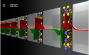
\includegraphics[height=3.5cm]{img/toc.pdf}
\end{tocentry}

\begin{document}

\newpage{}


% \section{Introduction}
% \label{sec:org2ea169d}
\linenumbers{}

\begin{abstract}
  The dielectric constant, which defines the polarization of
  the media, is a key quantity in condensed matter. It determines
  several electronic and optoelectronic properties important for a
  plethora of modern technologies, and its importance of 
  % from computer memory to field effect
  % transistors and communication circuits. Moreover, the importance of
  % the dielectric constant in
  describing electromagnetic interactions through screening plays a
  critical role in understanding fundamental molecular
  interactions. Here we show that despite its fundamental
  transcendence, the dielectric constant does not define unequivocally
  the dielectric properties of two-dimensional (2D) materials due to
  the locality of their electrostatic screening. Instead, the
  electronic polarizability correctly captures the dielectric nature
  of a 2D material which is united to other physical quantities in an
  atomically thin layer. Being a quantity with unique definition, the
  electronic polarizability overcomes the disadvantage of uncertainty
  posed by the effective dielectric constant model conventionally used
  to described screening in 2D material systems.  Furthermore, we
  reveal a long-sought universal formalism where electronic,
  geometrical and dielectric properties are intrinsically correlated
  through the polarizability opening the door to probe quantities yet
  not directly measurable including the real covalent thickness of a
  layer. Lastly, we unify the concept of dielectric properties in any
  material dimension finding a global dielectric anisotropy index
  defining their controllability through dimensionality.
\end{abstract}

\pagebreak{}

\section{Introduction}
\label{sec:introduction}

The dielectric constant $\varepsilon$ (also known as the relative permittivity) 
plays a crucial role in bridging various fundamental material
properties, such as bandgaps\cite{Moss_1950_relation,Moss_1985_n_Eg}, 
optical absorption\cite{kittel_2005_introduction} and 
conductivities\cite{Dressel_2001_electrodynamics}   
with elemental interactions. 
The central place of $\varepsilon$ in solid-state physics drives the analysis of several phenomena 
where is common to classify a material accordingly to its ability to screen an 
electric field $\boldsymbol{E}$ in terms of insulators, metals and semiconductors. Such definitions determine a broad range of 
condensed matter physics, as well as in related fields in chemistry and materials science. 
The ability to compute and measure $\varepsilon$ in bulk materials is well established via different 
theoretical \cite{Adler_1962,Hybertsen_1987} and experimental techniques \cite{palik_1998handbook} of distinct flavors
% where the probe of the dielectric properties 
% is made through an external electric field. 
%
Despite its obvious appeal, however, it is still unknown whether such quantity can determine the 
% electronic and
dielectric properties of two-dimensional (2D) materials \cite{Novoselov_2016}.  
%
The confined nature of such atomically-thin 2D crystals associated
with the attenuated and anisotropic character of the dielectric
screening
\cite{Keldysh_1979_eps_multi,Sharma_1985,Low_2014_screening_BP,Cudazzo_2011_screening_2D,Bechstedt_2012,Cudazzo_2010_screen2D,Nazarov_2015_2D_3D}
have generated long-standing debates whether the dielectric constant
truly represents dielectric features of such low-dimensional systems,
% or it can be used only as an
% additional parameter from the bulk-counterparts.
The controversy of
$\varepsilon$ values reported by both theoretical and experimental
approaches can be widely seen throughput literature\cite{Li_2016},
where the variation of $\varepsilon$ can be more than one order of
magnitude. As a consequence, several key physical parameters that
scales with $\varepsilon$, such as the exciton binding energy and
Debye screening length, cannot be reliably estimated due to the
discrepancy of reported $\varepsilon$ values. In this letter, we give
a thorough study of the underlying issue. Using \textit{ab initio}
simulations of a model system, we demonstrate that the macroscopic
dielectric constant strongly depends on the size of the superlattice,
making it unsuitable to describe the screening of a 2D material. On
the contrary, by analyzing the formalism of dielectric tensors, we
propose that the electronic polarizability is the true descriptor
which uniquely captures the dielectric nature of 2D materials. The 2D
electronic polarizability has unique definition, which overcomes the
disadvantage of ambiguity compared with the conventionally used
effective dielectric medium model for 2D materials. Moreover, we show
the universal scaling relations for in- and out-of-plane 2D electronic
polarizabilities with the electronic and geometric information of the
2D material. The concept of electronic polarizabilities bridges the
gap between the dielectric properties of 2D and 3D systems, and can be
extended to characterize the dielectric anisotropy for any material
dimensions.


%%
%%

\section{Results and discussions}
\label{sec:results-discussions}

\subsection{Lattice-dependency of macroscopic dielectric constant}
\label{sec:latt-depend-macr}

We first approach the discrepancy of macroscopic dielectric constant
of 2D materials, by showing that the current definition of
$\varepsilon$ used in layered materials is ill defined.  This can be
viewed in a model system as illustrated
in Figure \ref{fig-1}, where an isolated 2D material is placed in
the \textit{xy}-plane of a periodically repeating superlattice (SL)
with a length $L$ along the \textit{z}-direction separating the cell
images. The static macroscopic dielectric tensor from the superlattice
$\varepsilon_{\mathrm{SL}}^{pq}$, is determined through fundamental
electrostatics by the response of the polarization density
$\boldsymbol{P}^{p}$ under small perturbative external field
$\boldsymbol{E}^{q}$, where $p$, $q$ are the directions of
polarization and electric field,
respectively~\cite{Dressel_2001_electrodynamics}:
\begin{subequations}
  \begin{eqnarray}
      \label{eq:def-eps-1}
    &\varepsilon_{\mathrm{SL}}^{pq} &= \kappa^{pq} +
                                 {\displaystyle \frac{\partial \boldsymbol{P}^{p}}
                                 {\varepsilon_{0} \partial \boldsymbol{E}^{q}}} \\
          \label{eq:def-eps-2}
    &\boldsymbol{P}^{p} &=  {\displaystyle \frac{\boldsymbol{u}^{p}}{\Omega}}
                          = {\displaystyle \frac{{\displaystyle
          \int_{\mathrm{SL}} \rho(\boldsymbol{r}) \boldsymbol{r}^{p} d^{3}\boldsymbol{r}}}
                          {AL}}
  \end{eqnarray}
\end{subequations}
where $\kappa$ is the dielectric tensor of the environment,
$\boldsymbol{u}$ is the total dipole moment within the SL, $\rho$ is
the spatial charge density, $\Omega=AL$ is the volume of the
supercell, $A$ is the \textit{xy}-plane area of the SL and
$\varepsilon_{0}$ is vacuum permittivity. Here we limit out study on
the electronic contribution to the macroscopic dielectric constant
where the dipole $\boldsymbol{P}$ comes from the displacement of
electrons under external field.  On the other hand, the ionic
contribution to $\varepsilon_{\mathrm{SL}}$ that comes from
displacement of atomic nuclei is not covered in this due to its
complex dependency on several factors including phonon
dispersion~\cite{Sohier_2017} as well as lattice
symmetry~\cite{Laturia_2018}, which requires separated discussions.
The symmetry of 2D materials lead to the negligible off-diagonal
elements of the dielectric tensor ($p \neq q$), while and diagonal
elements $\varepsilon_{\mathrm{SL}}^{xx}$,
$\varepsilon_{\mathrm{SL}}^{yy}$ and $\varepsilon_{\mathrm{SL}}^{zz}$
can be different \cite{Sohier_2016}.  Considering that the 2D material
is placed in vacuum ($\kappa^{pp} = 1$ and $\kappa^{pq} = 0$), we can
distinguish two components of $\varepsilon_{\mathrm{SL}}$, namely the
in-plane ($\varepsilon_{\mathrm{SL}}^{\parallel}$) and out-of-plane
($\varepsilon_{\mathrm{SL}}^{\perp}$) dielectric constants, where
$\varepsilon_{\mathrm{SL}}^{\parallel} =
(\varepsilon_{\mathrm{SL}}^{xx} + \varepsilon_{\mathrm{SL}}^{yy})/2$
and
$\varepsilon_{\mathrm{SL}}^{\perp} = \varepsilon_{\mathrm{SL}}^{zz}$.
The absence of bonding perpendicular to the plane confines the induced
dipoles along the \textit{z}-direction within a range of $\sim{}$5--6
\AA{} into the vacuum (Figure \ref{fig-1}{\textbf a} and Supplementary
Figure \ref{SI-fig:rho-profile}).
%
%
Under a certain external field, when $L$ increases, the confinement of
the induced dipole moment $\boldsymbol{u}$ causes the integral in the
numerator of Eq.~\ref{eq:def-eps-2} to be saturated, when the
separation is large enough such that dipole moment from periodic
images do not mutually interfere. On the other hand, the increase of
$L$ in the denominator of Eq.~\ref{eq:def-eps-2} dilutes the polarization density, and in turn makes both
$\varepsilon^{\parallel}_{\mathrm{SL}}$ and
$\varepsilon^{\perp}_{\mathrm{SL}}$ dropping to
unity when $L$ is infinitely large.
% In the case of bulk materials
% such physical dependence is well described given the periodicity of
% the 3D crystal throughout the space.
%
%since this volume is used to represent the crystal 
%periodically throughout the space.  
%
%
% In the case of 2D materials, however, such repetition is artificial along the direction 
% perpendicular to the plane.
Despite of the simplicity of this argument, any calculation performed
using such definition will intrinsically depend on the magnitude of
$L$, an artificial parameter introduced by simulation system. This
dependence can be clearly demonstrated by plotting
$\varepsilon^{\parallel}_{\mathrm{SL}}$ and
$\varepsilon^{\perp}_{\mathrm{SL}}$ calculated from density functional
theory (DFT) (see {\it Theoretical Methods} for details) as a function
of $L$ for P\={6}m2 transition metal dichalcogenides (TMDCs),
2H-MX$_{2}$, where M=Mo, W and X=S, Se, Te (top panels of Figure
\ref{fig-1}{\textbf b} and \ref{fig-1}{\textbf c}, respectively). To
get a better description of the electronic band structure, the
calculations of dielectric properties were performed at the level of
Heyd-Scuseria-Ernzerhof (HSE06) hybrid functional
\cite{Heyd_2003,Heyd_2006}.  Both components of the dielectric
constant decreases with $L$ as excepted. To rule out the possibility
that the result is affected by the choice of \textit{ab initio}
methods, we also performed simulations at higher levels of theory
using many-body techniques (G$_{0}$W$_{0}$), which invariably give
alike results (see Supplementary Figure \ref{SI-fig:GW-PBE-alpha}).
The lattice-size dependency also exists for dielectric function in the
frequency ($\omega$) domain. We carried out similar analysis for
frequency-dependent $\varepsilon^{\parallel}_{\mathrm{SL}}(\omega)$
and $\varepsilon^{\perp}_{\mathrm{SL}}(\omega)$ using different levels
of techniques, including Perdew-Burke-Ernzerhof (PBE)
exchange-correlation functional
\cite{Perdew_1996,Ernzerhof_1999,Paier_2005}, many-body Green function
method (G\textsubscript{0}W\textsubscript{0})~\cite{Hedin_1965} and
Bethe-Salpethe equation (BSE)~\cite{Onida_2002}, with increasing
accuracy of calculated optical properties (PBE $<$
G\textsubscript{0}W\textsubscript{0} $<$ BSE) due to including of
many-body screening and excitonic effects (details see Supplementary
Section \ref{SI-ssec:gw}). Despite various levels of theory involved,
the magnitude of dielectric functions calculated universally decreases
with $L$ over the frequency domain.  These results indicate that
quantities that depend on
$\varepsilon^{\parallel}_{\mathrm{SL}}(\omega)$ and
$\varepsilon^{\perp}_{\mathrm{SL}}(\omega)$, including the optical
absorption (abs., equivalent to $\mathrm{Im}(\varepsilon_{\mathrm{SL}}(\omega))$), refractive index ($n$,  $\sim{}\sqrt{\mathrm{Re}(\varepsilon_{\mathrm{SL}})}$) and electron energy loss spectrum (EELS, equivalent to $-1 / \mathrm{Im}(\varepsilon_{\mathrm{SL}}(\omega))$), suffers the same
deficiencies as $\varepsilon_{\mathrm{SL}}$ for 2D materials. This
simple model system explains the origin of the discrepancy of
dielectric constant values reported in previous
literature~\cite{Li_2016}.
%
%%%
%
% We observe that neither
% $\varepsilon^{\parallel}_{\mathrm{SL}}$ nor
% $\varepsilon^{\perp}_{\mathrm{SL}}$ converges with $L$ due to fact
% that the long-range Coulomb interaction could not be completed
% screened within the range of magnitudes computationally accessible
%.
%
%
%As a result, the $L$-dependency of $\varepsilon_{\mathrm{SL}}$ makes
%it impractical to represent the dielectric nature of a 2D material
%both theoretically and experimentally, because the size of vacuum
%layer must always be considered. 
%

\subsection{The electronic polarizability of 2D materials}
\label{sec:electr-polar-2d}

To solve the problem described above, we need to find the
$L$-independent alternative of $\varepsilon_{\mathrm{SL}}$, which is
related to both electrostatic and optical properties of a 2D
material~\cite{Matthes_2016}. By multiplying Eq.~\ref{eq:def-eps-2}
with $L$, we obtain the sheet polarization density that is,
$\boldsymbol{\mu}_{\mathrm{2D}}^{p} =\boldsymbol{u}^{p}/A$, in
direction $p$. Following the discussion in the previous section,
$\boldsymbol{\mu}_{\mathrm{2D}}^{p}$ becomes independent of lattice
size when $L$ is large enough, due to the saturation of
$\boldsymbol{u}^{p}$.
%
Similar to the molecular polarizability \cite{Israelachvili_2011}, we
can define a 2D electronic polarizability $\alpha_{\mathrm{2D}}$ which
characterizes the ability to induce dipole moment of a 2D material. It
is associated with $\boldsymbol{\mu}_{\mathrm{2D}}$ through:
$\boldsymbol{\mu}_{\mathrm{2D}}^{p} = \sum_{q}
\alpha_{\mathrm{2D}}^{pq} \boldsymbol{E}_{\mathrm{loc}}^{q}$
\cite{T_bik_2004}, where $\boldsymbol{E}_{\mathrm{loc}}$ is the local
electric field causing the polarization. At $L \rightarrow \infty$
limit, $E_{\mathrm{loc}}$ can be solved using electrostatic boundary
conditions of slab geometry \cite{Markel_2016}. The continuity of the
electric field along the in-plane direction gives
$\boldsymbol{E}^{\parallel}_{\mathrm{loc}}=\boldsymbol{E}^{\parallel}$,
while for the out-of-plane component, the dipole screening yields
$\boldsymbol{E}_{\mathrm{loc}}^{\perp}=\boldsymbol{E}^{\perp}+\boldsymbol{\mu}_{\mathrm{2D}}^{\perp}/L$
\cite{Meyer_2001_dipole_slab,T_bik_2004}, where
$\boldsymbol{E}^{\parallel}$ and $\boldsymbol{E}^{\perp}$ are the
external field in the in-plane and out-of-plane directions,
respectively. Combining with Eqs. \ref{eq:def-eps-1} and
\ref{eq:def-eps-2},
$\alpha_{\mathrm{2D}}^{\parallel}$ and $\alpha_{\mathrm{2D}}^{\perp}$
can be related with $\varepsilon_{\mathrm{SL}}^{\parallel}$ and
$\varepsilon_{\mathrm{SL}}^{\perp}$, respectively:
%
%
\begin{subequations}
\begin{eqnarray}
  \label{eq:alpha-para-def}
  &\varepsilon_{\mathrm{SL}}^{\parallel} &= 1 + \frac{\alpha_{\mathrm{2D}}^{\parallel}}{\varepsilon_{0}L}\\
  \label{eq:alpha-perp-def}
  &\varepsilon_{\mathrm{SL}}^{\perp} &= \left(1 - {\displaystyle \frac{\alpha_{\mathrm{2D}}^{\perp}}{\varepsilon_{\mathrm{0}} L}} \right)^{-1}
\end{eqnarray}
\end{subequations}
% 20191003-16:00
% As pointed before, as we limit the discussion on electronic contributions to the dielectric properties, $\alpha_{\mathrm{2D}}$ characterizes the polarizability of electron cloud of a 2D materials.
% refers to the electronic polarizability (the polarizability of the
% electron cloud \cite{Israelachvili_2011}).

%
%
Using these relations, we show the calculated
$\alpha_{\mathrm{2D}}^{\parallel}$ and $\alpha_{\mathrm{2D}}^{\perp}$
of the selected TMDCs as a function of $L$ in the bottom panels of
Figure \ref{fig-1}b and \ref{fig-1}c, respectively.  In contrast to
$\varepsilon_{\mathrm{SL}}^{\parallel}$ and
$\varepsilon_{\mathrm{SL}}^{\perp}$, We observe that both
$\alpha_{\mathrm{2D}}^{\parallel}$ and $\alpha_{\mathrm{2D}}^{\perp}$
reach convergence when $L$ exceeds 10 \AA and 15 \AA,
respectively. Such result is in good agreement with the spatially
localized induced dipole moment of a 2D materials as shown in
Supplementary Figure~\ref{SI-fig:rho-profile}.
%
%
% Interestingly, we can use Eqs.\ref{eq:alpha-para-def} and
% \ref{eq:alpha-perp-def} to reproduce the trends noticed in the top
% panels in Figure\ref{fig-1}{\textbf b} and \ref{fig-1}{\textbf c} for
% $\varepsilon_{\mathrm{SL}}^{\parallel}$ and
% $\varepsilon_{\mathrm{SL}}^{\perp}$ as a function of $L$ around a
% centered magnitude of $\alpha_{\mathrm{2D}}^{\parallel}$ and
% $\alpha_{\mathrm{2D}}^{\perp}$
% (Figure \ref{fig-1}\textbf{d}-\textbf{e}).
% A similar curve profile is obtained in both components of the dielectric constant including the much 
% abrupt variation of $\varepsilon_{\mathrm{SL}}^{\perp}$ with $L$ which is due to 
% interlayer interactions.
%\todo[inline]{The original claim of this sentence, that $\varepsilon_{\mathrm{SL}}^{\perp}$ varies more due to interlayer interactions is not 100\% true. I think it is better not to explicitly mention this.}
Such relations can also be used to remove the dependence on $L$ for
frequency-dependent $\varepsilon^{\parallel}_{\mathrm{SL}}(\omega)$
and $\varepsilon^{\perp}_{\mathrm{SL}}(\omega)$, generating
lattice-independent electronic polarizability
$\alpha^{\parallel}_{\mathrm{SL}}(\omega)$ and
$\alpha^{\perp}_{\mathrm{SL}}(\omega)$ in the frequency domain,
respectively (details see Supplementary Section \ref{SI-ssec:gw}).
%
% 
% 
% 
% 
These findings indicate that the electronic polarizability $\alpha_{\mathrm{2D}}$ captures the essence
of the dielectric properties of 2D materials. In contrast to the ill-defined macroscopic $\varepsilon_{\mathrm{SL}}$, $\alpha_{\mathrm{2D}}$ has unique definition, and does not suffer from the dependency on the lattice size.
More discussions about the choice of the
2D polarizability, comparison with other methods, simulations at the
frequency-dependent domain can be found in Supplementary Section
\ref{SI-ssec:gw}.

\subsection{Comparison with effective dielectric model (EDM)}
\label{sec:comp-with-effect}

Apart from the 2D electronic polarizability proposed here, it is worth
mentioning that the effective dielectric model (EDM) is widely used in
literature to treat the 2D material as a slab with an effective
dielectric tensor $\varepsilon_{\mathrm{2D}}$ and thickness
$\delta^{*}_{\mathrm{2D}}$. Such method can be found in both
experimental and theoretical studies, such as to interpret
ellipsometry data
\cite{graphene-epsilon10,Duesberg14,Chiang13,Kong14}, reflectance /
transmission spectra \cite{Li_2014, Yoffe-Wilson69}, optical
conductance \cite{Matthes_2016} and many-body interactions
\cite{Sohier_2016,Meckbach_2018} of 2D materials. The EDM allows
applying physical laws of bulk systems directly to 2D materials using
$\varepsilon_{\mathrm{2D}}$. However, there are several drawbacks of
such approach, first of all, the wavevector($q$)-dependency of
dielectric screening in 2D
sheets~\cite{Cudazzo_2011_screening_2D,Olsen_2016_hydrogen,Trolle_2017_eps_subst}
is not captured. More severely, here we show that, due to the
uncertainty of $\delta^{*}_{\mathrm{2D}}$, the calculated
$\varepsilon_{\mathrm{2D}}$, in particular its out-of-plane component,
is extremely sensitive to the choice of $\delta^{*}_{\mathrm{2D}}$,
making such model questionable.

The basic assumption of EDM can be
seen in the inset of Figure~\ref{fig-1}\textbf{e}, where the macroscopic
$\varepsilon_{\mathrm{SL}}$ is considered to be contributed by (i) a
2D slab with effective dielectric constant $\varepsilon_{\mathrm{2D}}$
and thickness $\delta^{*}_{\mathrm{2D}}$ and (ii) vacuum spacing with
distance $L-\delta^{*}_{\mathrm{2D}}$. Using the effective medium theory
(EMT)~\cite{Aspnes_1982,Markel_2016}, the relation between
$\varepsilon_{\mathrm{SL}}$ and $\varepsilon_{\mathrm{2D}}$ can be
expressed using capacitance-like
equations~\cite{Matthes_2016,Laturia_2018} :
\begin{subequations}
  \begin{eqnarray}
    \label{eq:emt-1}
    {\displaystyle \varepsilon_{\mathrm{SL}}^{\parallel}} &= {\displaystyle \frac{\delta^{*}_{\mathrm{2D}}}{L} \varepsilon_{\mathrm{2D}}^{\parallel} + \left(1 - \frac{\delta^{*}_{\mathrm{2D}}}{L} \right)}\\
     \label{eq:emt-2}
    {\displaystyle \frac{1}{\varepsilon_{\mathrm{SL}}^{\perp}}} &= {\displaystyle \frac{\delta^{*}_{\mathrm{2D}}}{L} \frac{1}{\varepsilon_{\mathrm{2D}}^{\perp}} + \left(1 - \frac{\delta^{*}_{\mathrm{2D}}}{L} \right)}
  \end{eqnarray}
\end{subequations}
In principle, both the values of $\varepsilon_{\mathrm{2D}}$ and
$\delta^{*}_{\mathrm{2D}}$ are unknown for a certain 2D material. To
minimize the modeling error, we used non-linear least-square fitting
to extract $\varepsilon_{\mathrm{2D}}$ and $\delta^{*}_{\mathrm{2D}}$ of
selected 2H TMDCs simultaneously from \textit{ab initio}
$\varepsilon_{\mathrm{SL}}$ -- $L$ data in
Figure~\ref{fig-1}\textbf{b} and \ref{fig-1}\textbf{c} (details see
Supplementary Figure~\ref{SI-fig:rescale-prb}). The fitted values of
the slab thickness, $\delta_{\mathrm{2D}}^{\parallel, \mathrm{fit}}$
and $\delta_{\mathrm{2D}}^{\perp, \mathrm{fit}}$ from in-plane and
out-of-plane data, respectively, are shown in Supplementary
Table~\ref{SI-tab:delta-L-DFt}.
%
% As seen in Figure
% \ref{fig-emt}\textbf{b}, the estimation error of the thickness
% estimated from different directions is around 0.06$\sim{}$0.27
% \AA{}.
%
Although the uncertainty only corresponds to several percent of the
interlayer spacing in the bulk counterparts of these 2D materials, its
influence on the calculated values
$\varepsilon_{\mathrm{2D}}^{\parallel}$ and
$\varepsilon_{\mathrm{2D}}^{\perp}$ is significant. We estimated the
dispersion of $\varepsilon_{\mathrm{2D}}^{\parallel}$ and
$\varepsilon_{\mathrm{2D}}^{\perp}$ if $\delta^{*}_{\mathrm{2D}}$
deviates from the best fitted value by $\pm{}$2.5 \AA{}, as shown in
Figures \ref{fig-1}\textbf{d} and \ref{fig-1}\textbf{e},
respectively. $\varepsilon_{\mathrm{2D}}^{\parallel}$ decays linearly
with $\delta^{*}_{\mathrm{2D}}$,
while strikingly, the value $\varepsilon_{\mathrm{2D}}^{\perp}$ spans
over more than one order of magnitude. The sensitivity of
$\varepsilon_{\mathrm{2D}}^{\perp}$ to $\delta^{*}_{\mathrm{2D}}$
explains the discrepancy in literature that both
isotropic~\cite{Sohier_2016} and highly
anisotropic~\cite{Matthes_2016,Laturia_2018}
$\varepsilon_{\mathrm{2D}}$ tensors for 2D materials under the EDM are
reported. As a consequence, the estimated values of
$\varepsilon_{\mathrm{2D}}$, in particular its out-of-plane component,
is highly questionable.

On the contrary, the proposed $\alpha_{\mathrm{2D}}$ approach does not
suffer from such deficiencies, despite its relatively simple
formalism. The relative uncertainty of $\alpha_{\mathrm{2D}}$ is
generally at the order of 10\textsuperscript{-4} (Supplementary
Figure~\ref{SI-fig:alpha-converg}). In addition, the calculation of
$\alpha_{\mathrm{2D}}$ technically simpler than
$\varepsilon_{\mathrm{2D}}$: (i) $\alpha_{\mathrm{2D}}$ can be
achieved using single-point calculation of macroscopic dielectric
tensor, while $\varepsilon_{\mathrm{2D}}$ requires non-linear fitting
of multiple $\varepsilon_{\mathrm{SL}}$ -- $L$ data points; (ii) the
values of $\alpha_{\mathrm{2D}}$ typically converge well for large $L$
($>$20 \AA{}), while $\varepsilon_{\mathrm{2D}}$ suffers from the
uncertainty as described above.

%\subsection*{Polarizability as the fundamental variable}
%\label{sec:first-principles}

%We consider 

\subsection{Universal scaling laws of $\alpha_{\mathrm{2D}}$}
\label{sec:univ-scal-laws}

For bulk materials, pioneering works from the 1950s have demonstrated
empirical equations between $\varepsilon$ and the bandgap
$E_{\mathrm{g}}$, including the
Moss~\cite{Moss_1950_relation,Moss_1985_n_Eg,Finkenrath_1988} or
Ravindra~\cite{Ravindra_1980_model,Ravindra_1979_eps_Eg} relations.
Such universal relations, if exist in the context of
$\alpha_{\mathrm{2D}}$, would be of high importance for studying and
predicting the screening of 2D materials.  Inspired by the random
phase approximation (RPA) theory \cite{Adler_1962} within the
$\mathbf{k} \cdot \mathbf{p}$
formalism\cite{kittel_2005_introduction,Jiang_2017_Eg_Eb}, we propose the universal relations for $\alpha_{\mathrm{2D}}^{\parallel}$ and $\alpha_{\mathrm{2D}}^{\perp}$,
depending on the electronic and geometric information of a 2D material (see
Supplementary Section \ref{SI-sec:theory-1} for details):
% \begin{subequations}
% \begin{eqnarray}
% \label{eq:2D-Moss-para}
  % &\alpha_{\mathrm{2D}}^{\parallel} &=C^{\parallel} E_{g}^{-1} \\
  % \label{eq:2D-Moss-perp}
  % &\alpha_{\mathrm{2D}}^{\perp} & =C^{\perp} \hat{\delta}_{\mathrm{2D}}
% \end{eqnarray}
% \end{subequations}
\begin{subequations}
\begin{eqnarray}
\label{eq:2D-Moss-para}
  &E_{\mathrm{g}} &= C^{\parallel} \alpha_{\mathrm{2D}}^{\parallel} \\
  \label{eq:2D-Moss-perp}
  &\hat{\delta}_{\mathrm{2D}} & = C^{\perp} \alpha_{\mathrm{2D}}^{\perp} 
\end{eqnarray}
\end{subequations}
where $E_{\mathrm{g}}$ is the fundamental electronic bandgap and
$\hat{\delta}_{\mathrm{2D}}$ is the intrinsic thickness of the 2D
layer, with coefficients
$C^{\parallel} = {\displaystyle \frac{2 \pi}{Ne^2}}$
\cite{Jiang_2017_Eg_Eb}, where $N$ is a pre-factor associated with the
band degeneracy, and $C^{\perp} = {\varepsilon_{0}}^{-1}$. It is worth
noting, unlike the parameter $\delta^{*}_{\mathrm{2D}}$ that is
artificially assigned within the EDM picture (see previous section),
$\hat{\delta^{*}_{\mathrm{2D}}}$ can be uniquely defined by
$\alpha_{\mathrm{2D}}^{\parallel}$, a quantity that can be
computationally and experimentally determined. Despite of the
simplicity of Eqs. \ref{eq:2D-Moss-para} and \ref{eq:2D-Moss-perp},
they generalize direct relationships between the electronic polarizability and
the electronic / structural properties for any 2D material in a new
framework.

Next, we show that these equations are valid for the current
library of known layered materials involving different lattice
symmetry, element composition, optical and electronic properties.
%
A high-throughput screening performed on different families of TMDCs
(MX\(_{\text{2}}\), where M is a metal in groups 4, 6, 10, and X=O, S,
Se, Te) and phases (P\={6}m2, P3m1), metal monochalcogenides
(Ga\textsubscript{2}S\textsubscript{2},
Ga\textsubscript{2}Se\textsubscript{2}), cadmium halides (CdX$_2$,
X=Cl, I), hexagonal boron nitride (BN), graphene derivatives
(fluorographene (C\textsubscript{2}F\textsubscript{2}), graphane
(C\textsubscript{2}H\textsubscript{2})), phosphorene
(P\textsubscript{4}) and thin layer organic-inorganic perovskites
(ABX\textsubscript{3}) (Figure \ref{fig-3}{\textbf a}) shows that our
method enables full correlation between these disparate variables.
Figure \ref{fig-3}{\textbf b} compares the calculated fundamental
bandgap $E_{\mathrm{g}}$ (blue dots) and 2D electronic
polarizabilities (bar plots) of all the 2D materials investigated,
covering a wide spectrum range from far-infrared to ultraviolet.  Note
from dimension analysis, it is more intuitive to express the
polarizability as $\alpha_{\mathrm{2D}}/(4 \pi \varepsilon_{0})$,
which has unit of \AA{}. We find that
$\alpha_{\mathrm{2D}}^{\parallel}$ has a general descending trend when
$E_{\mathrm{g}}$ increases, while no apparent correlation between
$\alpha_{\mathrm{2D}}^{\perp}$ and $E_{\mathrm{g}}$ is observed (see
Supplementary Section \ref{SI-sec:pol-2D-Eg}).  We then examine
Eqs. \ref{eq:2D-Moss-para} and \ref{eq:2D-Moss-perp} using the
polarizabilities by first-principle calculations.  Figure
\ref{fig-3}\textbf{c} shows
$(4 \pi \varepsilon_{0})/\alpha_{\mathrm{2D}}^{\parallel}$ (in
\AA{}$^{-1}$) as a function of $E_{\mathrm{g}}$ (in eV) for the 2D
materials investigated (circle dots) at HSE06 level.  A linear
regression coefficient of $R^{2}=0.84$ indicates a strong correlation
between bandgaps and polarizabilities as predicted in
Eq. \ref{eq:2D-Moss-para}.  We also discover that the linearity
between $(4 \pi \varepsilon_{0})/\alpha_{\mathrm{2D}}^{\parallel}$ and
$E_{\mathrm{g}}$ (measured by the $R^{2}$ value) is higher when the
bandgap is calculated using the HSE06 hybrid functional compared with
that from PBE exchange-correlation functional (see Supplementary
Section \ref{SI-sec:pol-2D-Eg} and Supplementary Figure
\ref{SI-fig:alpha-Eg-diff}) which suggests that higher levels of
theory are needed to precisely predict bandgaps.  A detailed benchmark
of Eqs.~\ref{eq:2D-Moss-para} and \ref{eq:2D-Moss-perp} using
different bandgaps, databases, and levels of calculation can be seen
in Supplementary Section~\ref{SI-sec:gpaw}.


We further examine the validity of Eq.~\ref{eq:2D-Moss-perp}, i.e.,
the relation between $\alpha_{\mathrm{2D}}^{\perp}$ and the thickness
of a 2D material. To test if the quantity $\hat{\delta_{\mathrm{2D}}}$
is physical, we choose the ``covalent'' thickness
$\delta_{\mathrm{cov}}$ of a 2D material as a
comparison. $\delta_{\mathrm{cov}}$ is defined as the longest distance
along the \textit{z}-direction between any two atom nuclei plus their covalent
radii:
%
%
\begin{equation}
  \label{eq:cov-thick}
  \delta_{\mathrm{cov}} = \mathrm{max}(|z^{i} - z^{j}|
  + r^{i}_{\mathrm{cov}} + r^{j}_{\mathrm{cov}})
\end{equation}
where $i$, $j$ are atomic indices in the 2D material and
$r_{\mathrm{cov}}^{i}$ is the covalent radius of atom $i$ (Figure
\ref{fig-3}{\textbf d} inset). As shown in Figure~\ref{fig-3}{\textbf
  d}, $\alpha_{\mathrm{2D}}^{\perp}/\varepsilon_{0}$ (or equivalently,
$\hat{\delta}_{\mathrm{2D}}$) is very close to $\delta_{\mathrm{cov}}$
with a good linear correlation of $R^{2}=0.98$. This result indicates
a strong relation between $\alpha_{\mathrm{2D}}^{\perp}$ and the
geometry of the 2D layer, which can be approximated by
$\delta_{\mathrm{cov}}$. Similar to the molecular polarizability which
characterizes the volume of the electron cloud of an isolated molecule
\cite{Israelachvili_2011},
$\alpha_{\mathrm{2D}}^{\perp}/\varepsilon_{0}$ is also naturally
related to the characteristic thickness of the electron cloud of 2D
material. Supplementary Section
\ref{SI-ssec:theory-1-perp-fundamental} shows an explanation of this
behavior from fundamental electrostatics and why
$\alpha_{\mathrm{2D}}^{\perp} / \varepsilon_{0}$ is close to
$\delta_{\mathrm{cov}}$. Our proposed definition of
$\hat{\delta_{\mathrm{2D}}}$ of a 2D material based on
Eq. \ref{eq:2D-Moss-perp} may have impact
on some long-existing controversies about the experimental thickness
of 2D materials~\cite{Shearer_2016}, through the
measurable quantity $\alpha_{\mathrm{2D}}^{\perp}$
\cite{Antoine_1999,Cherniavskaya_2003,Krauss_1999_EFM}.
% 
%

To rule out the possibility that our conclusion are limited by the
number of materials used at HSE06 level, we further validate
Eqs. \ref{eq:2D-Moss-para} and \ref{eq:2D-Moss-perp} using two
different 2D material databases \cite{Haastrup_2018,Mounet_2018}, from
which we extracted the dielectric properties of over 300 compounds
calculated at the PBE level, and superimpose with our results in
Figure \ref{fig-3}{\textbf c} and \ref{fig-3}{\textbf d}. Although the
calculated dielectric properties may be different due to different
choice of functionals as well as underestimation of the bandgap
compared with the more accurate HSE06 functionals
\cite{Van_Dyck_2017}, similar linear trends can be observed for both
$\alpha^{\parallel}_{\mathrm{2D}}$ and $\alpha_{\mathrm{2D}}^{\perp}$
with the linear coefficient very close to the HSE06 results, which
further proves the validity of our proposed relations. We have also
searched for additional relations between the 2D polarizabilities with
other physical quantities, including the effective carrier mass,
quantum capacitance (density of states) and total atomic
polarizabilities with no apparent correlations being found
(Supplementary Section \ref{SI-sec:gpaw-3}).

\subsection{Application in multilayer and bulk systems}
\label{sec:apply-electr-polar}
The concept of electronic polarizability is not limited to monolayer
materials, and can be applied to multilayer and bulk systems as
well. For a 2D material stack composed of $N$ layers, we can define
the electronic polarizability $\alpha_{\mathrm{NL}}$ similar to
Eqs. \eqref{eq:alpha-para-def} and \eqref{eq:alpha-para-def}. Note
$\alpha_{\mathrm{NL}}(N=1)$ is equivalent to $\alpha_{\mathrm{2D}}$.
Figure \ref{fig-4}\textbf{a} and \ref{fig-4}\textbf{b} show
$\alpha_{\mathrm{NL}}^{\parallel}$ and $\alpha_{\mathrm{NL}}^{\perp}$
as functions of $N$ for the selected 2H TMDCs,
respectively. Interestingly, we find that in all cases,
$\alpha_{\mathrm{NL}}$ exhibits nearly ideal linear relation with
$\alpha_{\mathrm{2D}}$, such that
$\alpha_{\mathrm{NL}}^{\parallel}= N \alpha_{\mathrm{2D}}^{\parallel}$
and $\alpha_{\mathrm{NL}}^{\perp}= N
\alpha_{\mathrm{2D}}^{\perp}$. Due to the relatively small
electric applied (0.01 eV/\AA{}), the interlayer interactions within
the stack are negligible. Under such circumstances, $\alpha_{\mathrm{2D}}$ of individual layers is additive, which leads to the following general relation:
\begin{equation}
  \label{eq:alpha-nl}
  \alpha_{\mathrm{NL}}^{p} = \sum_{i=1}^{N} \alpha_{\mathrm{2D, i}}^{p},\quad p=\parallel\ \mathrm{or}\ \perp
\end{equation}
where $\alpha_{\mathrm{2D, i}}$ is the electronic polarizability of
layer $i$, and $p$ is the direction of polarization. This relation can
be further used to calculate screening inside 2D heterostructures
\cite{Kumar_2016_jpcc,Andersen_2015_dielec_vdWH}.
%
%
%

We further look into the bulk systems. In a bulk layered material stacked by layers with equilibrium
inter-layer distance $L_{\mathrm{Bulk}}$, we define the polarizability
of individual layer $\alpha_{\mathrm{2D}}(L=L_{\mathrm{Bulk}})$ as
$\alpha_{\mathrm{Bulk}}$. Inspired by Eqs. \ref{eq:alpha-para-def} and
\ref{eq:alpha-perp-def}, the dielectric constants
$\varepsilon^{\parallel}_{\mathrm{Bulk}}$ and
$\varepsilon^{\perp}_{\mathrm{Bulk}}$ of the bulk layered material can
be reconstructed by $\alpha_{\mathrm{Bulk}}^{\parallel}$ and
$\alpha_{\mathrm{Bulk}}^{\perp}$ (Figure \ref{fig-4}{\textbf a}) as:
%
%
\begin{subequations}
\begin{align}
  \label{eq:3D-para}
  \varepsilon^{\parallel}_{\mathrm{Bulk}}
  &= 1 + \frac{\alpha_{\mathrm{Bulk}}^{\parallel}}{\varepsilon_{0} L_{\mathrm{Bulk}}}
  \approx 1 + \frac{\alpha_{\mathrm{2D}}^{\parallel}}{\varepsilon_{0} L_{\mathrm{Bulk}}} \\
  \label{eq:3D-perp}
  \varepsilon^{\perp}_{\mathrm{Bulk}}
  &= \left(1 - \frac{\alpha_{\mathrm{Bulk}}^{\perp}}{\varepsilon_{0} L_{\mathrm{Bulk}}}\right)^{-1}
  \approx \left(1 - \frac{\alpha_{\mathrm{2D}}^{\perp}}{\varepsilon_{0} L_{\mathrm{Bulk}}}\right)^{-1}
\end{align}
\end{subequations}
%
%
Here we neglect the effect of the stacking order of the layers.  The
dielectric constant $\varepsilon$ although not well-defined for a
monolayer 2D material becomes applicable when the 2D layers are put
together.
%
We compare the values of
$\varepsilon_{\mathrm{bulk}}^{\parallel}$ and
$\varepsilon_{\mathrm{bulk}}^{\perp}$ from DFT calculations (\textit{y}-axis)
with those predicted using Eqs \ref{eq:3D-para} and \ref{eq:3D-perp}
(\textit{x}-axis) as shown in Figure \ref{fig-4}{\textbf b} and \ref{fig-4}{\textbf c}. 
Both HSE06 and PBE datasets give almost identical results.  
%
We observe that
$\varepsilon_{\mathrm{bulk}}^{\parallel}$ values calculated by DFT and
predicted by Eq. \ref{eq:3D-para} are in good agreement with a linear
regression slope of 1.01 and $R^2$ of 0.97. Conversely,
$\varepsilon_{\mathrm{bulk}}^{\perp}$ values predicted from
Eq. \ref{eq:3D-perp} agree well with the DFT-calculated values when
$E_{\mathrm{g}}>4$ eV, while the deviation becomes larger when
$E_{\mathrm{g}}$ reduces. The above results indicate that
$\alpha^{\parallel}_{\mathrm{Bulk}}$ can generally be estimated from
its 2D counterpart, while $\alpha^{\perp}_{\mathrm{Bulk}}$ differs due
to the interlayer coupling and overlap between induced
dipoles\cite{Andersen_2015_dielec_vdWH,Laturia_2018}. 
%With a better model describing
%$\alpha_{\mathrm{bulk}}^{\perp}$ as function of $\alpha_{\mathrm{2D}}^{\perp}$ and
%the degree of interlayer coupling, the dielectric transition from 2D
%to 3D would be smoothly described.

\subsection{Unified geometric represenation of $\alpha_{\mathrm{2D}}$}
\label{sec:unif-geom-repr}

%
Lastly, we demonstrate that both $\alpha_{\mathrm{2D}}^{\parallel}$
and $\alpha_{\mathrm{2D}}^{\perp}$ can be unified using a geometric
picture. In merit of the unit analysis,
$\alpha_{\mathrm{2D}}^{\parallel}$ and $\alpha_{\mathrm{2D}}^{\perp}$
both have unit of $4\pi\varepsilon_{0} \cdot$[Length]. In other words,
they represent in- and out-of-plane characteristic lengths,
respectively. It is well-known that the in-plane screened
electrostatic potential (Keldysh potential) $V(r)$ from a point charge
as a function of distance $r$:
$V(r) = {\displaystyle \frac{e}{4 \alpha_{\mathrm{2D}}^{\parallel}}}
\left[H_{0}({\displaystyle \frac{2\varepsilon_{0}
      r}{\alpha_{\mathrm{2D}}^{\parallel}}}) - Y_{0}( {\displaystyle
    \frac{2
      \varepsilon_{0}r}{\alpha_{\mathrm{2D}}^{\parallel}}})\right]$
\cite{Keldysh_1979_eps_multi,Pulci_2014}, where $H_{0}$ is the Struve
function and $Y_{0}$ is the Bessel function of second kind, is
associated with the in-plane screening radius
$r_{0}^{\parallel}=\alpha_{\mathrm{2D}}^{\parallel}/(2
\varepsilon_{0})$, such that $V(r,r/r^{\parallel}_{0} \gg 1)$ reduces
to the simple Coulomb potential in vacuum. Combining with the result
that $\alpha_{\mathrm{2D}}^{\perp}/\varepsilon_{0}$ characterizes the
thickness of a 2D material, we can view the dielectric screening of a
point charge sitting in the middle of a 2D material as an ellipsoid
with the radii of principle axes to be
$r_{0}^{\parallel} = \alpha_{\mathrm{2D}}^{\parallel}/(2
\varepsilon_{0})$ and
$r_{0}^{\perp} = \alpha^{\perp}_{\mathrm{2D}}/(2 \varepsilon_{0})$,
respectively, as illustrated in Figure~\ref{fig-ellip}\textbf{a}.
This is analog to the polarizability ellipsoid picture of molecules
used in spectroscopy \cite{Banwell_1994}. The polarizability ellipsoid
for a 2D material is in general ultra flat, with
$r_{0}^{\parallel} \gg r_{0}^{\perp}$, as demonstrated by the examples
of group 6 2H TMDCs (Figure~\ref{fig-ellip}\textbf{a} and
~\ref{fig-ellip}\textbf{b}). The polarizability ellipsoid picture
provides further insights into the physical nature of
$\alpha_{\mathrm{2D}}$: $r_{0}^{\parallel}$ is close to the exciton
radius that confined within the 2D plane~\cite{Pulci_2014}, which is
generally larger for a smaller bandgap semiconductor, and can be
converted through the exciton binding energy as proposed in
Refs. \citenum{Olsen_2016_hydrogen,Jiang_2017_Eg_Eb}
Eq. \ref{eq:2D-Moss-para}. On the other hand, $r_{0}^{\perp}$ may be
indirectly deduced from Stark effect
\cite{Pedersen_2016,Klein_2016,Roch_2018}.
% and the low-frequency Raman
% scattering modes of 2D materials \cite{Tan_2012,Zhang_2013}.

%\subsection{Bridging the 2D and 3D Dielectric Properties}
%\label{sec:2D-3D}

Inspired by the polarizability ellipsoid model, we show that a general picture of the dielectric properties in
any dimension can be drawn by studying the dielectric
anisotropy. We define the dielectric anisotropy index $\eta$ as:
\begin{equation}
  \label{eq:anisotropy}
  \begin{aligned}[t]
    \eta =
    \begin{cases}
      {\displaystyle \min_{i \neq j}}
      {\displaystyle
        \left(\frac{\varepsilon^{ii}}{\varepsilon^{jj}}\right)},
      \ \mathrm{Bulk\ Materials}\\
      {\displaystyle \min_{i \neq j}}
      {\displaystyle
        \left(\frac{\alpha_{\mathrm{2D}}^{ii}}{\alpha_{\mathrm{2D}}^{jj}}\right)},
      \ \mathrm{2D\ Materials}\\
    \end{cases}
  \end{aligned}
\end{equation}
$\eta=1$ indicates the material has isotropic dielectric properties
while $\eta \to 0$ means the dielectric property is highly
anisotropic. Figure \ref{fig:aniso} shows the phase diagram of $\eta$
as function of $E_{\mathrm{g}}$ for 2D materials and their bulk
counterparts. Interestingly, the 2D materials (blue triangles) can be
clearly distinguished from the bulk layered materials (orange squares)
with the boundary line determined to be
$\eta =0.048 (E_{\mathrm{g}}/ \mathrm{eV})+0.087$. The much lower
$\eta$ values for 2D materials compared with their bulk counterparts
indicates a high dielectric anisotropy, which is responsible for the
unique 2D optoelectronic properties, such as the electrostatic
transparency phenomena\cite{Liluhua_2014,Tian_2016,Li_2018} and the large exciton
binding energies
\cite{Pulci_2014,Tran_2014,Chernikov_2014_EB_MoS2_2D3D,Berkelbach_2013}. From
Eqs. \ref{eq:2D-Moss-para}, \ref{eq:2D-Moss-perp} and
\ref{eq:anisotropy} we can see $\eta$ is roughly proportional to
$\delta \cdot E_{\mathrm{g}}$, which explains the observation that
$\eta$ for 2D materials increase almost linearly with
$E_{\mathrm{g}}$, since the layer thickness $\delta$ (mostly 3--10
\AA{}) of the 2D materials investigated varies much less than
$E_{\mathrm{g}}$ (0.1--7 eV) (Figure \ref{fig-3}b and
\ref{fig-3}c). Further analysis shows that the dielectric anisotropy
index of any bulk layered material $\eta_{\mathrm{Bulk}}$ obeys
$\eta_{\mathrm{Bulk}} \geq {\displaystyle \frac{4
    \eta_{\mathrm{2D}}}{(\eta_{\mathrm{2D}}+1)^{2}}} \geq
\eta_{\mathrm{2D}}$, where $\eta_{\mathrm{2D}}$ is the anisotropy
index of corresponding 2D layer (see additional details in
Supplementary Section \ref{SI-sec:aniso}), which is the basis for the
separation of bulk and 2D regimes in the $\eta-E_{\mathrm{g}}$ phase
diagram.  For comparison, we also superimpose the dielectric
anisotropy indices of common semiconducting materials in other
dimensions (details see Supplementary Section \ref{SI-sec:aniso}) on
the phase diagram in Figure \ref{fig:aniso}. Bulk covalent (3D,
e.g. Si, GaN) and 0D (fullerenes) semiconductors show isotropic
dielectric properties, scattered on the line $\eta=1$. On the other
hand, reduced dimensionality increases the dielectric anisotropy of
materials such as planar organic semiconductor (OSc, 1D-2D,
e.g. CuPc), carbon nanotube (CNT, 1D), linear OSc (0D-1D,
e.g. polyacene and polyacetylene). Interestingly, most of these
materials also scatter along the boundary line separating the bulk and
2D regimes, indicating the criteria distinguishing 2D (more
anisotropic) and bulk layered materials (more isotropic) from the
$\eta-E_{\mathrm{g}}$ diagram, can also be applied to other
dimensions. From the phase diagram, we can see that 2D and bulk
layered materials (also including 2D van der Waals heterostructure
(vdWH) \cite{Novoselov_2016}), provides more flexibility in
controlling the dielectric and electronic properties, compared with
semiconductors in other dimensions.

%
%\subsection{Implications for Experiments}
%\todo[inline]{Wait for comments from JC and MC.}


\section{Conclusion}
%\label{sec:org5fd1f1a}
%\todo[inline]{To be changed later when everything fixed}

Our results show that the 2D electronic polarizability
$\alpha_{\mathrm{2D}}$ is a local variable determining the dielectric
properties of 2D materials.  There exist well defined relationships
between $\alpha_{\mathrm{2D}}$ and other quantities hidden in the
electronic properties.  According to our analysis, simple scaling
equations involving bandgaps and layer thicknesses can be used to
describe both dielectric and electronic features at the same
footing. A dielectric anisotropy index is found relating any material
dimension with its controllability.  Thus, our results suggest that
the challenge of understanding the dielectric phenomena is in general
a geometrical problem mediated by the bandgap. We believe the
principles presented here will benefit both fundamental understanding
of 2D materials as well as rational device design and optimization.




\section{Theoretical Methods}
\label{sec:org8457dbb}

Simulations were carried out using plane-wave density functional
theory package VASP \cite{Kresse_1993,Kresse_1996_1,Kresse_1996_2}
using the projector augmented wave (PAW) approach with GW
pseudopotentials \cite{Kresse_1999_pseudopotentials}. Band gaps were
calculated using the Heyd-Scuseria-Ernzerhof hybrid functional (HSE06)
\cite{Heyd_2003,HSE_2006}, with spin orbit coupling (SOC) explicitly
included. The geometries were converged both in cell parameters and
ionic positions, with forces below 0.04 eV/\AA. To ensure the accuracy
of dielectric property of monolayer, a vacuum spacing of $>$ 15 \AA~is
used. A k-point grid of \(7\times7\times1\) was used to relax the
superlattice, with an initial relaxation carried out at the
Perdew-Burke-Ernzerhof
(PBE)\cite{Perdew_1996,Ernzerhof_1999,Paier_2005_PBE}
exchange-correlation functional level and a subsequent relaxation
carried out at HSE06 level, allowing both cell parameters and ionic
positions to relax each time. In VASP, the tag PREC=High was used,
giving a plane wave kinetic energy cutoff of 30\% greater than the
highest given in the pseudopotentials used in each material. This
guarantees that absolute energies were converged to a few meV and the
stress tensor to within 0.01 kBar.  Calculation of the macroscopic
ion-clamped dielectric tensor were carried out with an
18$\times$18$\times$1 k-grid and electric field strength of 0.001
eV/\AA.  Local field effect corrections are included at the
exchange-correlation potential $V_{\mathrm{xc}}$ at both PBE and HSE06
levels. The materials from Ref.\citenum{Haastrup_2018} for comparison
were choses with the GW bandgap larger than 0.05 eV. Bulk layered
materials were constructed by relaxing the c-axis length of
corresponding monolayer material with the interlayer van der Waals
(vdW) interactions calculated by non-local vdW correlation
functional\cite{Lee_2010_vdFD2}.  The dielectric properties of bulk
layered materials using VASP were calculated at HSE06 level with
18$\times$18$\times$6 k-grid with same parameter as for monolayer,
while the dielectric properties of bulk counterparts of
Ref.~\citenum{Haastrup_2018} are calculated at PBE level with a
k-point density of 10~\AA$^{-1}$. Local field effect corrections are
also used for the dielectric properties of bulk systems.


\section{Data Availability}
The data that support the findings of this study are available from
the corresponding author upon reasonable request.



\bibliography{ref}

% \section{Figures}
\label{sec:org34cbe74}
\begin{figure}[H]
\centering
\includegraphics[width=0.75\linewidth]{img/fig1.pdf}
\caption{\label{fig-1} \textbf{2D polarizability and the breakdown of
    effective dielectric model
    (EDM)} % \textbf{2D polarizability as the
  % true descriptor of the dielectric nature of 2D materials.}
  \textbf{a}. 3D illustration of the spatial distribution of the
  charge density change $\Delta \rho(z)$ along the z-direction for
  monolayer 2H-MoS\textsubscript{2} in a periodic superlattice under
  external eletric field of 0.01 V/\AA{}.  The green and red regions
  represent negative and positive induced charges, respectively. The
  macroscopic $\varepsilon_{\mathrm{SL}}^{\parallel}$ and
  $\varepsilon_{\mathrm{SL}}^{\perp}$ are influenced by the lattice
  size $L$, while the 2D polarizabilities
  $\alpha_{\mathrm{2D}}^{\parallel}$ and
  $\alpha_{\mathrm{2D}}^{\perp}$ are invariant with lattice size
  \textbf{b}.  $\varepsilon^{\parallel}_{\mathrm{SL}}$ (top) and
  $\alpha_{\mathrm{2D}}^{\parallel}$ (bottom) as functions of $L$ for
  the 2H TMDCs. \textbf{c}.  $\varepsilon^{\perp}_{\mathrm{SL}}$ (top)
  and $\alpha_{\mathrm{2D}}^{\perp}$ (bottom) as functions of $L$ for
  the 2H TMDCs. The polarizabilities in \textbf{b} and \textbf{c} are
  constant when $L>$15 \AA{}, compared with the $L$-dependence of
  $\varepsilon_{\mathrm{SL}}$. On the other hand, the EDM approach
  which usually used in literature to extract the effective 2D
  dielectric constant $\varepsilon_{\mathrm{2D}}$, fails to produce
  consistent results, estimation uncertainty of the effective layer
  thickness $\delta^{*}_{\mathrm{2D}}$, causes huge variations of
  $\varepsilon_{\mathrm{2D}}^{\parallel}$ (\textbf{d}) and
  $\varepsilon_{\mathrm{2D}}^{\perp}$ (\textbf{e}).
  % HSE06 functional is used in all plots.
}
\end{figure}

% \begin{figure}[H]
%   \centering
%   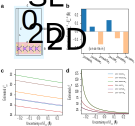
\includegraphics[width=0.75\linewidth]{img/fig-emt-uncertainty.pdf}
%   \caption{\label{fig-emt} \textbf{Failure of the effective 2D
%       ``dielectric constant'' picture based on the effective medium
%       theory (EMT)}. \textbf{a}.  Scheme of the EMT picture where an
%     effective 2D ``dielectric constant'' $\varepsilon_{\mathrm{2D}}$
%     is extracted from $\varepsilon_{\mathrm{SL}}$, which depends on
%     the thickness $\delta_{\mathrm{2D}}$ of the 2D material that is
%     not well-defined. \textbf{b}.  Estimation error between
%     $\delta_{\mathrm{2D}}^{\parallel, \text{fit}}$ and
%     $\delta_{\mathrm{2D}}^{\perp, \text{fit}}$ from non-linear fitting
%     of \textit{ab initio} $\varepsilon_{\mathrm{SL}} - L$ data for selected
%     2D TMDCs. The uncertainty of
%     $\delta_{\mathrm{2D}}$ causes considerable variation of estimated
%     $\varepsilon_{\mathrm{2D}}^{\parallel}$ (\textbf{c}.) and in
%     particular $\varepsilon_{\mathrm{2D}}^{\perp}$ (\textbf{d}.).  }
% \end{figure}

% \begin{figure}[htbp]
% \centering
% \includegraphics[width=0.8\linewidth]{./img/fig2.pdf}
% \caption{\label{fig-2} The elements and 3D structures of the 2D
  % materials investigated in this study.}
% \end{figure}

\begin{figure}[H]
\centering
\includegraphics[width=0.7\linewidth]{img/fig2.pdf}
\caption{\label{fig-3} \textbf{The universal scaling relation of the
    dielectric nature of 2D materials}. \textbf{a}. The structures of
  the 2D materials investigated in this
  study. \textbf{b}. $\alpha_{\mathrm{2D}}^{\parallel}$,
  $\alpha_{\mathrm{2D}}^{\perp}$ (bar plots) and $E_{\mathrm{g}}$
  (blue dots) for all the 2D materials studied.
  $\alpha_{\mathrm{2D}}^{\parallel}$ is observed to descend with
  increasing $E_{\mathrm{g}}$, while no apparent relation between
  $\alpha_{\mathrm{2D}}^{\perp}$ and $E_{\mathrm{g}}$ is
  observed. HSE06 functional is used to obtain the data. \textbf{c}.
  $(4\pi \varepsilon_{0})/\alpha_{\mathrm{2D}}^{\parallel}$ (in
  \AA{}$^{-1}$) as a function of $E_{\mathrm{g}}$, showing a linear
  correlation between each other. The energy range of visible light is
  shown in the background. \textbf{d}.
  $\alpha_{\mathrm{2D}}^{\perp}/(4\pi\varepsilon_{0})$ (in \AA{}) as a
  function of $\delta_{\mathrm{cov}}$ (definition schematically shown
  in the inset), showing a perfect linear relation with slope very
  close to $1/4\pi$ (i.e.
  $\alpha_{\mathrm{2D}}^{\perp} \approx \varepsilon_{0}
  \delta_{\mathrm{cov}}$ ). The universal scaling relation is also
  revealed using the data from Ref.~\citenum{Haastrup_2018} (squares),
  and Ref.~\citenum{Mounet_2018} (triangles) as superimposed on
  \textbf{c} and \textbf{d}.}
\end{figure}




% \begin{table}[H]
%   \centering
%   \caption{In-plane ($r_{0}^{\parallel}$) and out-of-plane
%     ($r_{0}^{\perp}$) radii of the polarizability ellipsoid of
%     selected 2D materials calculated from first principles
%     simulations. $r_{0}^{\parallel}$ is in general much larger than
%     $r_{0}^{\perp}$, which accounts for the highly anisotropic
%     dielectric nature of 2D materials.}
%   \label{tbl:radii}  
%   \begin{tabular}{lcc}
%     \hline
%     Material & $r_{0}^{\parallel} = \alpha_{\mathrm{2D}}^{\parallel}/2\varepsilon_{0}$ (\AA{}) &  $r_{0}^{\perp} = \alpha_{\mathrm{2D}}^{\perp}/2\varepsilon_{0}$ (\AA{})\\
%     \hline
%     2H-MoS$_{2}$ & 40.0 & 2.50 \\
%     2H-MoSe$_{2}$ & 45.5 & 2.72  \\
%     2H-MoTe$_{2}$ & 58.1 & 3.07  \\
%     2H-WS$_{2}$ & 35.7 & 2.46  \\
%     2H-WSe$_{2}$ & 41.0 & 2.71 \\
%     2H-WTe$_{2}$ & 53.5 &  3.17\\
%     \hline
%   \end{tabular}
% \end{table}

\begin{figure}[H]
\centering
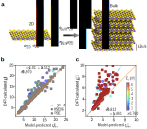
\includegraphics[width=0.9\linewidth]{img/fig4.pdf}
\caption{\label{fig-4} \textbf{Application of 2D polarizability to
    multilayer and bulk systems}.  \textbf{a}. Scheme for the 2D-3D
  transition. $\alpha$ in the 2D material is essentially equivalent to
  $\varepsilon$ in its bulk counterpart.  By applying the concept of
  electronic polarizability to multilayer 2D materials, the multilayer
  polarizabilities $\alpha_{\mathrm{NL}}^{\parallel}$ and
  $\alpha_{\mathrm{NL}}^{\perp}$ of selected 2D metal dichacolgenides
  as functions of number of layers $N$ are shown in \textbf{a} and
  \textbf{b}, respectively. Both $\alpha_{\mathrm{NL}}^{\parallel}$
  and $\alpha_{\mathrm{NL}}^{\perp}$ linearly scales with $N$ and the
  electronic polarizabilities of monolayer, indicating that
  $\alpha_{\mathrm{2D}}$ is an additive quantity under weak
  interacting regime. The 2D to 3D transition is further studied in
  \textbf{c} and \textbf{d}, where $\alpha_{\mathrm{2D}}$ of an
  monolayer 2D material is compared with its bulk counterpart
  $\varepsilon_{\mathrm{Bulk}}$. \textbf{c}
  $\varepsilon_{\mathrm{bulk}}^{\parallel}$ calculated from DFT
  (y-axis) compared with the predicted value from 2D
  $\alpha_{\mathrm{2D}}^{\parallel}$ (x-axis), showing good
  correlation. \textbf{d} $\varepsilon_{\mathrm{bulk}}^{\perp}$
  calculated from DFT (y-axis) compared with the predicted value from
  2D $\alpha_{\mathrm{2D}}^{\parallel}$ (x-axis). The predicted value
  is in good aggreement with the DFT calculation when
  $E_{\mathrm{g}}>4$ eV, due to minimal interlayer coupling. The
  comparisons in \textbf{b} and \textbf{c} are made based on both
  HSE06 (circles) and PBE (squares) functionals.}
\end{figure}

\begin{figure}[H]
  \centering
  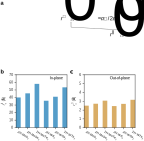
\includegraphics[width=0.8\linewidth]{img/fig-ellipsoid.pdf}
  \caption{\label{fig-ellip} \textbf{Geometric representation of the
      2D polarizability}. \textbf{a}. Scheme of the polarizability
    ellipsoid of a 2D material, with its in-plane
    ($r_{0}^{\parallel}$) and out-of-plane radii
    ($r_{\mathrm{0}}^{\perp}$) proportional to
    $\alpha_{\mathrm{2D}}^{\parallel}$ and
    $\alpha_{\mathrm{2D}}^{\perp}$, respectively.  The values of
    $r_{0}^{\parallel}$ and $r_{0}^{\perp}$ for selected 2D TMDCs are
    shown in \textbf{b} and \textbf{c}, respectively.  The
    polarizability ellipsoid is highly anisotropic with screening much
    larger at in-plane direction than out-of-plane direction.}
\end{figure}



\begin{figure}[H]
  \centering
  \includegraphics[width=1.01\linewidth]{img/fig5.pdf}
  \caption{\textbf{Phase diagram of dielectric anisotropy $\eta$ as
      function of bandgap $E_{\mathrm{g}}$}. The
    $\eta$-$E_{\mathrm{g}}$ values of 2D materials (blue triangle) and
    their bulk counterparts (orange square) can be distinguished by
    the line $\eta=0.048(E_{\mathrm{g}}/\mathrm{eV})+0.087$. $\eta-E_{\mathrm{g}}$ values of
    semiconducting materials in other dimensions are also superimposed
    for comparison. Isotropic dielectric property is observed for bulk
    covalent materials (3D, red triangle) and fullerenes (0D, green
    star), while reduced dimensional materials, including planar
    organic semiconductor(OSc, 1D-2D, brown triangle), carbon nanotube
    (CNT, magenta circle) and linear OSc (0D-1D, violet pentagon) are
    scattered along the boundary line. The dimensionality and
    structure of typical materials are shown along the axis on the
    right. Compared with other materials, 2D materials and their bulk
    counterparts provide more flexibility of controlling the
    dielectric anisotropy.}
  \label{fig:aniso}
\end{figure}

\end{document}
%%% Local Variables:
%%% mode: latex
%%% TeX-master: t
%%% End:
